\section{Implementation}
\subsection{Database}
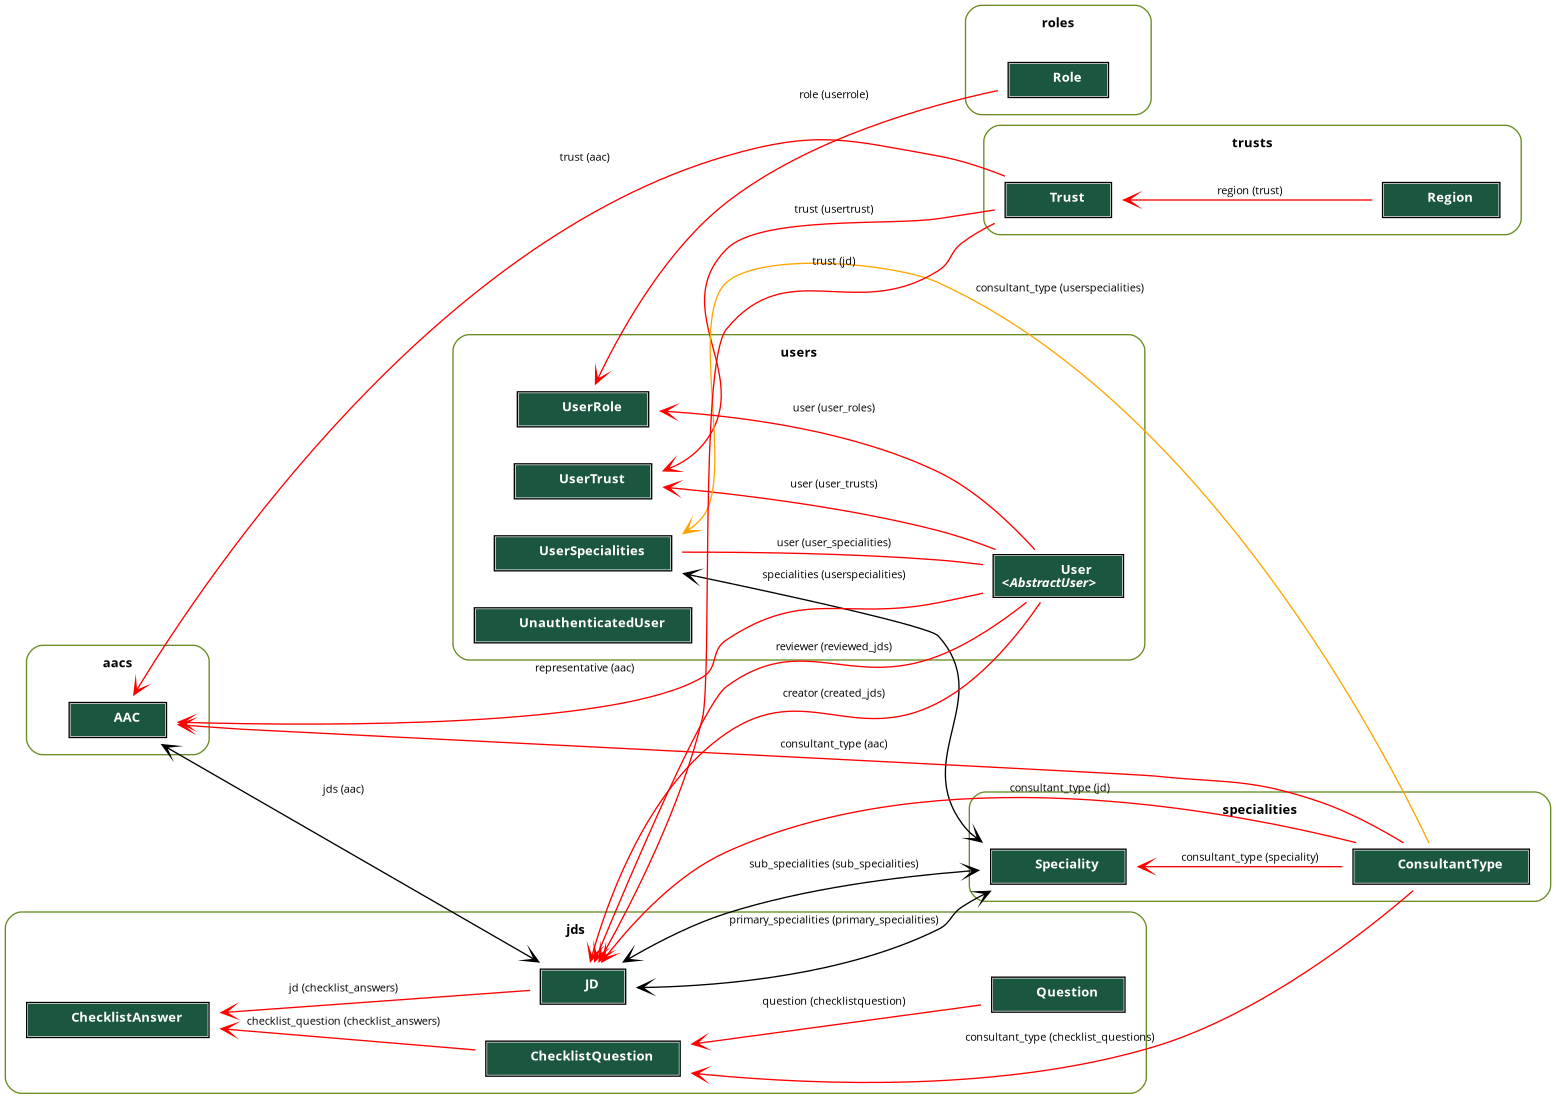
\includegraphics[width=\linewidth]{images/database.png}
This is the database at the moment. There is a lot more to be added.

\subsection{Dark Mode}
\begin{minipage}{0.77\textwidth} % Adjust the width of the text area
There are options to select light or dark mode, so there is the option of working later in the day without it impacting your sleep (SOURCE). 
\end{minipage}
\hfill
\begin{minipage}{0.2\textwidth} % Adjust the width of the image area
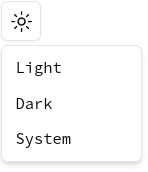
\includegraphics[width=\textwidth]{images/darkMode.png} % Adjust the width as necessary, using \textwidth scales the image to fit the minipage
\end{minipage}

\newpage
\begin{minipage}{0.46\textwidth} % Adjust the width of the image area
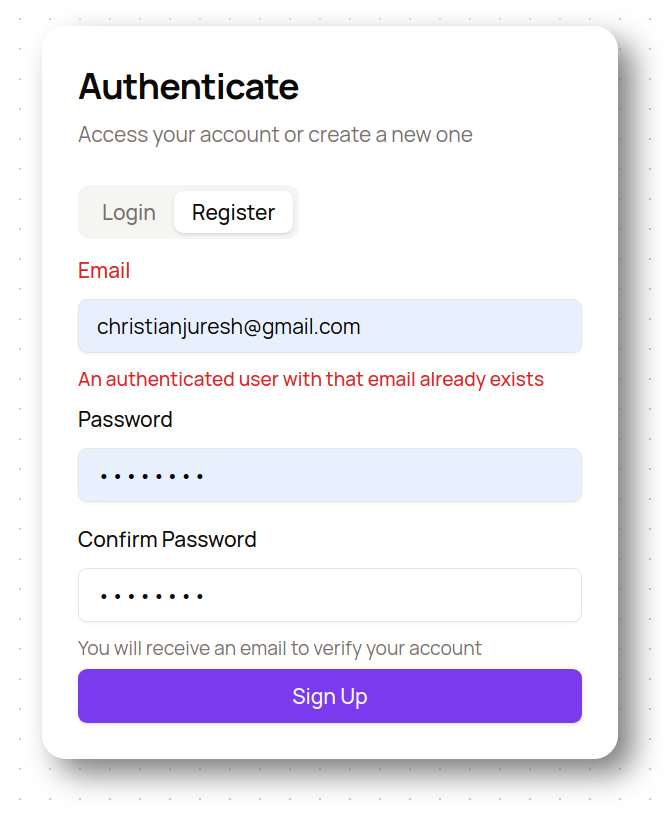
\includegraphics[width=\textwidth]{images/register.png} % Adjust the width as necessary, using \textwidth scales the image to fit the minipage
\end{minipage}
\hfill
\begin{minipage}{0.5\textwidth} % Adjust the width of the text area
\subsection{Registration}
    Users are met by an authentication page where they can choose to login or register. The registration form is validated in sveltekit using zod, and also communicates with the django backend to tell users if the email is already registered in the database. Upon registration, the user is sent an email by postmark to verify their account. When the link is pressed, the user is logged in and redirected to the profile page.
\end{minipage}

\begin{minipage}{0.3\textwidth}
\subsection{Profile}
    The profile page also includes zod validation, and users are able to select multiple roles to request validation for. A sidebar shows the roles and trusts the logged in user has been approved for.
\end{minipage}
\hfill
\begin{minipage}{0.66\textwidth}
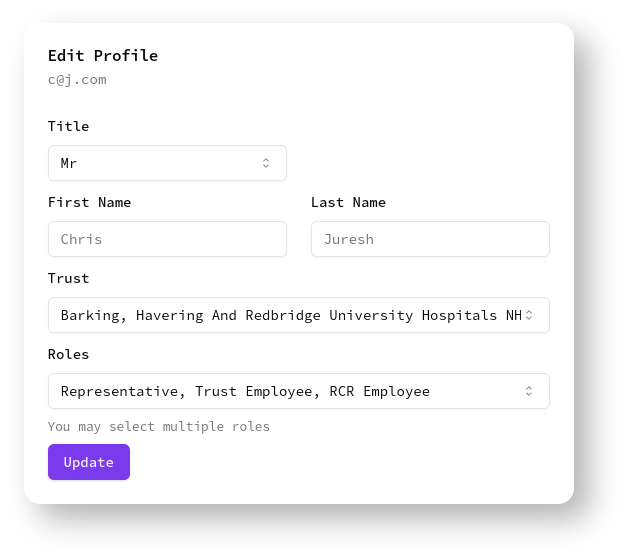
\includegraphics[width=\textwidth]{images/profile.png}
\end{minipage}

\subsection{Panel}
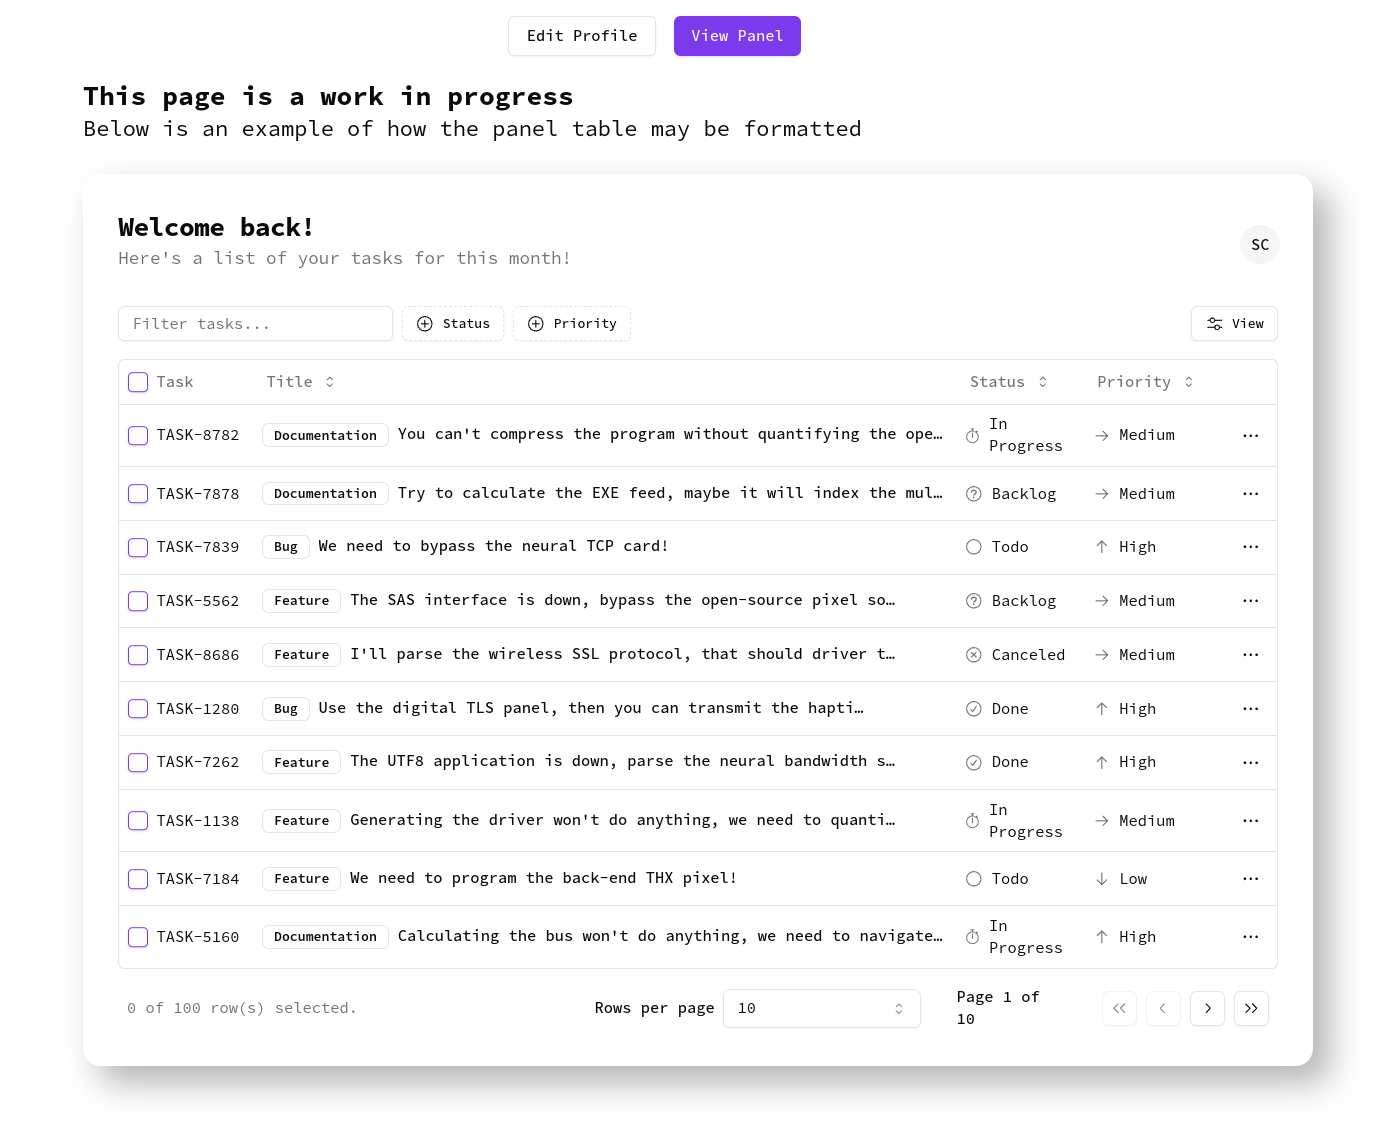
\includegraphics[width=\linewidth]{images/panel.png}
This page is incomplete. This is where the list of JDs and AACs will be displayed.